\begin{enumerate}[label=\thesubsection.\arabic*.,ref=\thesubsection.\theenumi]
\numberwithin{equation}{enumi}
\numberwithin{figure}{enumi}

\item Using Nyquist criterion, find out whether the following is stable or not.

\begin{equation}
    G(s) = \frac{100(s+5)}{s(s^2+4)(s+3)}
\end{equation}
\begin{equation}
    H(s) = 1
\end{equation}

\solution
Open loop transfer function (oltf):
\begin{equation} \label{eq:1}
    G(s)H(s) = \frac{100(s+5)}{s(s^2+4)(s+3)}
\end{equation}

Closed loop transfer function (cltf):
\begin{equation} \label{eq:2}
    \frac{G(s)}{1+G(s)H(s)}
\end{equation}

Nyquist Stability Criterion can be expressed as:
\begin{equation} \label{eq:3}
    Z = N + P
\end{equation}

where:
\begin{itemize}
    \item  Z = number of roots of 1+G(s)H(s) in right-hand side (RHS) of s-plane (It is also called zeros of characteristics equation).
    \item N = number of encirclement of critical point 1+j0 in the clockwise direction.
    \item P = number of poles of open loop transfer function (OLTF) [i.e. G(s)H(s)] in RHS of s-plane.
\end{itemize}
The above condition (i.e. Z=N+P) is valid for all the systems whether stable or unstable. 
\begin{itemize}
    \item The system is stable iff Z = 0.
\end{itemize}
The pole-zero plot of equation \ref{eq:1} is:
\begin{figure}[ht!]
        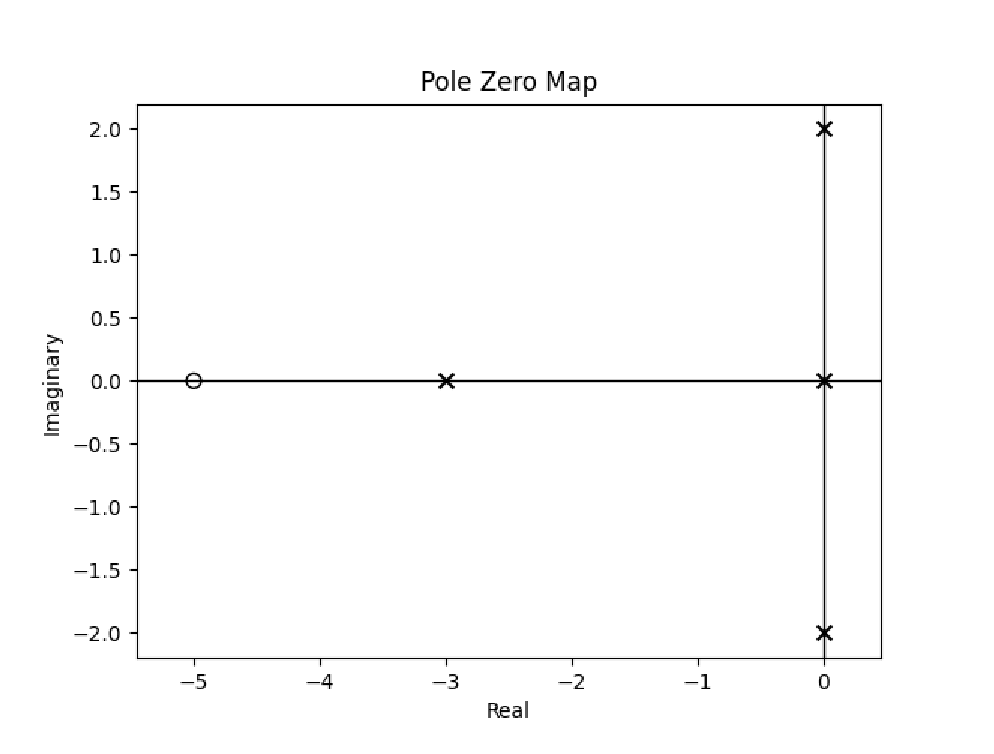
\includegraphics[width=\columnwidth]{./figs/ee18btech11025/pzG.eps}
        \caption{}
        \label{fig:pz}
\end{figure}

which gives P = 0.\\
Since there are poles on the imaginary axis of oltf \ref{eq:1}, the Nyquist contour will be (which encloses the right half s-plane)  : \\
\begin{figure}[ht!]
    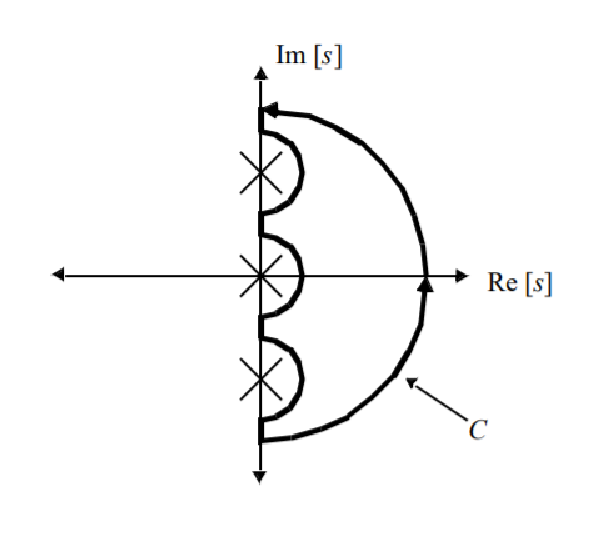
\includegraphics[width=\columnwidth]{./figs/ee18btech11025/splane.eps}
    \caption{}
    \label{fig:splane}
\end{figure}
The outer semi-circle C is infinitely large and smaller semicircle's radius goes to almost zero.

Plot of the Nyquist plot for equation \ref{eq:1} is:
\begin{figure}[ht!]
    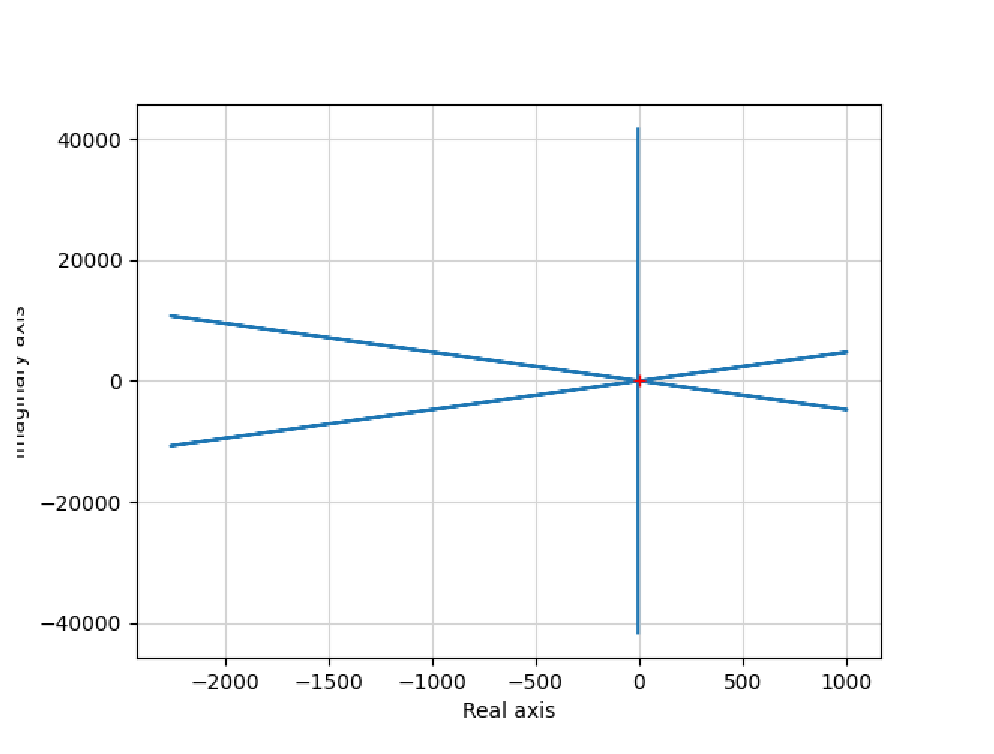
\includegraphics[width=\columnwidth]{./figs/ee18btech11025/g.eps}
    \caption{}
    \label{fig:nyqplot}
\end{figure}

\begin{figure}[ht!]
    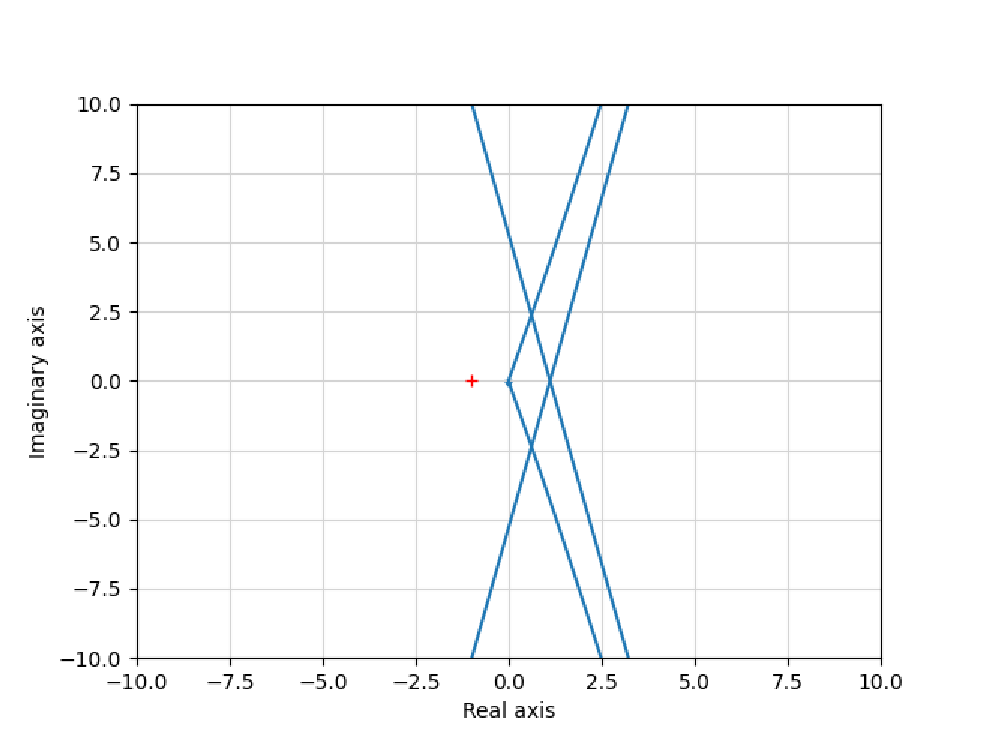
\includegraphics[width=\columnwidth]{./figs/ee18btech11025/g2.eps}
    \caption{Zoomed in}
    \label{fig:nyqplot1}
\end{figure}
\begin{itemize}
    \item The point -1+0j is encircled twice by the nyquist plot, once due to the semicircle at origin in fig: \ref{fig:splane} (which translates to infinitely big semicircle in Nyquist plot).
    \item Then due to poles on imaginary axis (which also translate to infinitely big semicircle).
\end{itemize}

which gives us N = 2.

Substituting values of P = 0 and N = 2 in equation \ref{eq:3}:
\begin{equation}
 \implies Z = 2
\end{equation}
This is verified using pole zero plot of 1+G(s)H(s): \\
\begin{figure}[ht!]
    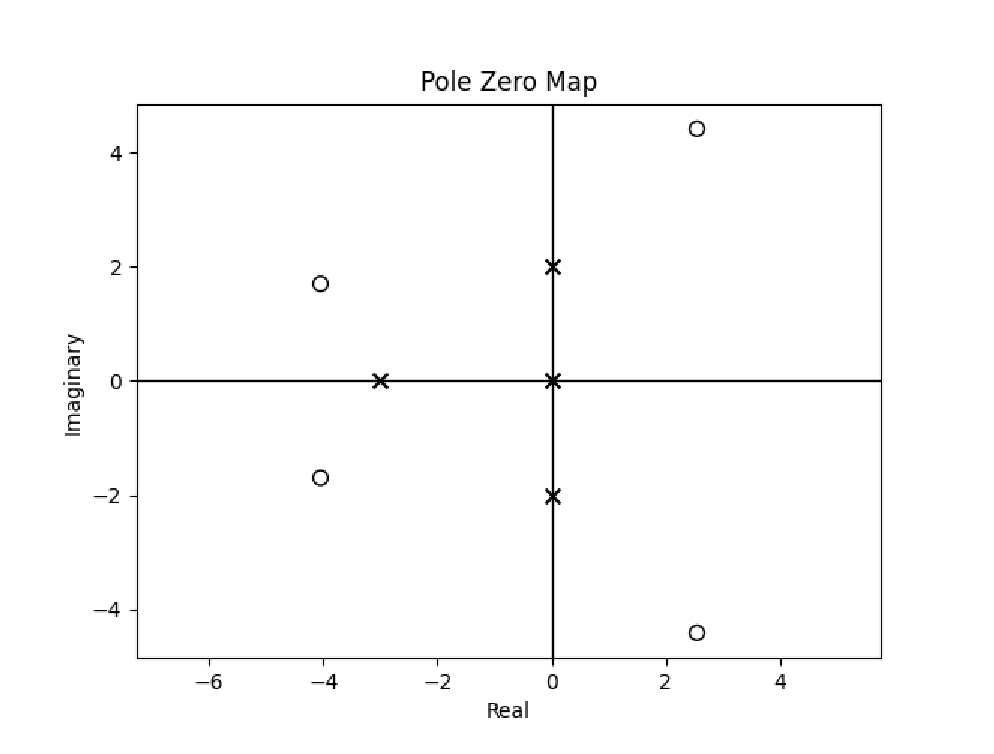
\includegraphics[width=\columnwidth]{./figs/ee18btech11025/pzG1.eps}
    \caption{}
    \label{fig:pz1}
\end{figure}
Two zeroes on RHP of s-plane i.e. Z=2. \\
Since $Z\neq0$, the system is unstable.

The following code plots the pole zero plot and the nyquist plot.
\begin{lstlisting}
    codes/ee18btech11025.py
\end{lstlisting}
\end{enumerate}